\documentclass[12pt, a4paper]{article}
\usepackage[margin=0.5in]{geometry}

\usepackage{color}
\usepackage[dvipsnames]{xcolor}
\usepackage{hyperref}
\hypersetup{
    colorlinks=true,
    linkcolor=blue,
    urlcolor=blue,
    linktoc=all
}


\usepackage{amsmath}
\usepackage{mathtools}
\usepackage{amssymb}
\usepackage{cancel}
\usepackage{bm}
\usepackage{dsfont}
\usepackage{graphicx}
\usepackage{graphics}
\usepackage{xfrac}
\usepackage{array}
\setcounter{MaxMatrixCols}{40}

\usepackage{enumerate}
\usepackage{enumitem}
\usepackage{multirow}

%inclusions carried over from past class homework formats
\usepackage{units}
\usepackage{fullpage}
\usepackage{alltt}
\usepackage{mathrsfs}
\usepackage{xcolor}
\usepackage{soul}

\usepackage{pgfplots}

\DeclarePairedDelimiter{\abs}{\lvert}{\rvert}
\newcommand*{\fontCourier}{\fontfamily{pcr}\selectfont}
\newcommand*\mean[1]{\overline{#1}}
\newcommand\scalemath[2]{\scalebox{#1}{\mbox{\ensuremath{\displaystyle #2}}}}

\setcounter{tocdepth}{5}
\setcounter{secnumdepth}{5}

\usepackage{pdfpages}
\usepackage{Sweave}
\begin{document}
%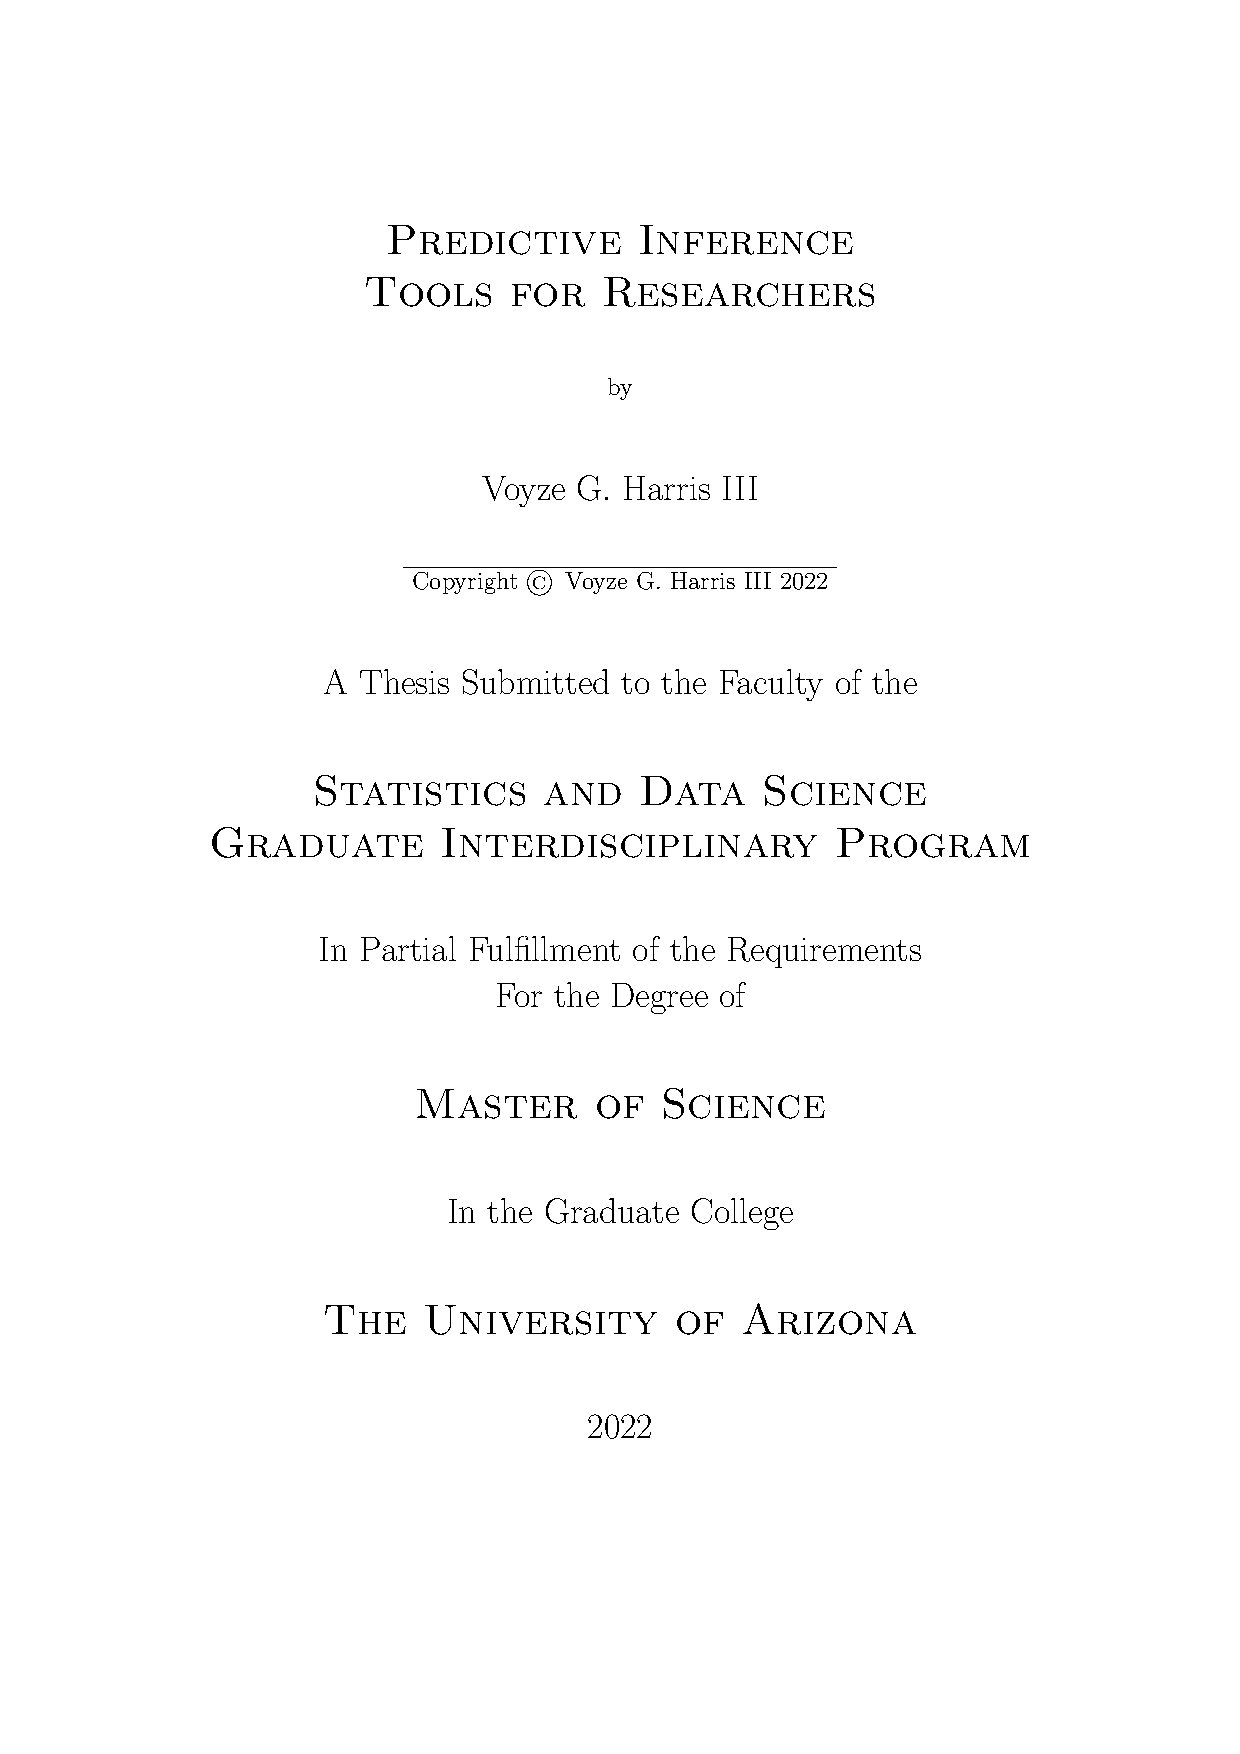
\includepdf{TitlePage_MastersThesis}
%
\includepdf{ThesisApprovalPage}
\Sconcordance{concordance:Regression.tex:Regression.Rnw:%
1 49 1 1 0 7 1 1 4 70 1 1 12 1 2 40 1 1 26 1 2 8 1}


%\tableofcontents
%\newpage


%%%%%%%%%%%%%%%%%%%%%%%%%%%%%%%%%
%%INTRODUCTION
%%%%%%%%%%%%%%%%%%%%%%%%%%%%%%%%%

(Hoff p. 149ff.)\\

Regression modeling is concerned with describing how the sampling istribution of one random variable $Y$ varies with another variable or set of variables $\mathbf{x} = \left(x_1,...,x_p\right)$.  Specifically, a regression model postulates a form for $p(y|\mathbf{x})$, the conditional distribution of $Y$ given $\mathbf{x}$.  Estimation of $p(y|\mathbf{x})$ is made using data $y_1,...,y_n$ that are gathered under a variety of conditions $\mathbf{x}_1,...,\mathbf{x}_n$.

The normal linear regression model specifies that, in addition to $E[Y|\mathbf{x}]$ being linear, the sampling variability around the mean is i.i.d. normal:

\begin{flalign*}
    \epsilon_1,...,\epsilon_n &\overset{\text{i.i.d}}{\sim} \text{normal}\left(0,\sigma^2\right)\\
    Y_i &= \beta^T \mathbf{x}_i + \epsilon_i
\end{flalign*}

This model provides a complete specification of the joint probability density of observed data $y_1,...,y_n$ conditional upon $\mathbf{x}_1,...,\mathbf{x}_n$ and values of $\beta$ and $\sigma^2$:

\begin{flalign}
    p\left(y_1,...y_n|\mathbf{x}_1,...,\mathbf{x}_n,\beta,\sigma^2\right) &= \prod_{i=1}^n p\left(y_i|\mathbf{x}_i,\beta,\sigma^2\right) \nonumber\\
    &= \left(2\pi\sigma^2\right)^{-n/2}\text{exp}\left\{-\frac{1}{2\sigma^2}\sum_{i=1}^n\left(y_i - \beta^T\mathbf{x}_i\right)^2\right\} \label{conditional_density}
\end{flalign}

Another way to write this joint probability density is in terms of the multivariate normal distribution:  Let $\mathbf{y}$ be the $n$-dimensional column vector $\left(y_1,...,y_n\right)^T$ and let $\mathbf{X}$ be the $n \times p$ matrix whose $i$th row is $\mathbf{x}_i = \left\{ x_{i,1}, x_{i,2}, ..., x_{i,p} \right\}$.  Then the normal regression model is

$$\{\mathbf{y}|\mathbf{X},\beta,\sigma^2\} \sim \text{multivariate normal}\left(\mathbf{X}\beta,\sigma^2\mathbf{I}\right),$$

where $\mathbf{I}$ is the $p \times p$ identity matrix and

\begin{equation*}
    \mathbf{X}\beta =
    \begin{pmatrix}
        \mathbf{x}_1 \\
        \mathbf{x}_2 \\
        \vdots  \\
        \mathbf{x}_n
    \end{pmatrix}
    \begin{pmatrix}
        \beta_1 \\
        \beta_2 \\
        \vdots \\
        \beta_p
    \end{pmatrix}
    =
    \begin{pmatrix}
        \beta_1 x_{1,1} + \cdots + \beta_p x_{1,p} \\
        \vdots \\
        \beta_1 x_{n,1} + \cdots + \beta_p x_{n,p} \\
    \end{pmatrix}
    =
    \begin{pmatrix}
        E\left[Y_1|\mathbf{\beta},\mathbf{x}_1\right] \\
        \vdots \\
        E\left[Y_n|\mathbf{\beta},\mathbf{x}_n\right] \\
    \end{pmatrix}
\end{equation*}

The density (\ref{conditional_density}) depends on $\beta$ through the residuals $\left(y_i - \beta^T\mathbf{x}_i\right)$.  We compute the ordinary least squares estimates

$$\hat{\beta}_{ols} = \left(\mathbf{X}^T\mathbf{X}\right)^{-1}\mathbf{X}^T\mathbf{y}$$

and

$$\hat{\sigma}^2_{ols} = \frac{SSR\left(\hat{\beta}_{ols}\right)}{(n-p)} = \frac{\sum\left(y_i - \hat{\beta}_{ols}^T x_i\right)^2}{(n-p)}.$$

\clearpage

\textit{Example:  Oxygen uptake (from Kuehl (2000), Hoff p. 149ff)}

Twelve healthy men who did not exercise regularly were recruited to take part in a study of the effects of two different exercise regimens on oxygen uptake.  Six of the twelve men were randomly assigned to a 12-week flat-terrain running program, and the remaining six were assigned to a 12-week step aerobics program.  The maximum oxygen uptake of each subject was measured (in liters per minute) while running on an inclined treadmill, both before and after the 12-week program.  Of interest is how a subject's change in maximal oxygen uptake may depend on which program they were assigned to.  However, other factors, such as age, are expected to affect the change in maximal uptake as well.  The results are shown here:

\includegraphics{Regression-002}

Hoff's regression model:

% \begin{flalign*}
%     Y_i &= \beta_1x_{i,1} + \beta_2x_{i,2} + \beta_3x_{i,3} + \beta_4x_{i,4} + \epsilon_i, \text{ where}\\
%     x_{i,1} &= 1 \text{ for each subject } i\\
%     x_{i,2} &= 0 \text{ if subject } j \text{ is on the running program, } 1 \text{ if on aerobic}\\
%     x_{i,3} &= \text{ age of subject } i\\
%     x_{i,4} &= x_{i,2} \times x_{i,3}
% \end{flalign*}

%\begin{subequations}
    \begin{align}
        Y_i &= \beta_1x_{i,1} + \beta_2x_{i,2} + \beta_3x_{i,3} + \beta_4x_{i,4} + \epsilon_i, \text{ where} \label{example_model}\\
        x_{i,1} &= 1 \text{ for each subject } i \nonumber \\
        x_{i,2} &= 0 \text{ if subject } j \text{ is on the running program, } 1 \text{ if on aerobic} \nonumber \\
        x_{i,3} &= \text{ age of subject } i \nonumber \\
        x_{i,4} &= x_{i,2} \times x_{i,3} \nonumber
    \end{align}
%\end{subequations}

% \begin{subequations}
% \begin{align}
% \frac{\mathrm{d} x}{\mathrm{d} t} &=\sigma(y-x)\label{eqn:line-1} \\
% \frac{\mathrm{d} y}{\mathrm{d} t} &=x(\rho-z)-y\label{eqn:line-2} \\
% \frac{\mathrm{d} z}{\mathrm{d} t} &=x y-\beta z
% \end{align}
% \label{eqn:all-lines}
% \end{subequations}
%
% Look at the first line \ref{eqn:line-1}, and now look at the second line \ref{eqn:line-2}. They are both part of the whole system \ref{eqn:all-lines}.

Under this model the conditional expectations of $Y$ for the two different levels of $x_{i,1}$ are

\begin{flalign*}
    E[Y|\mathbf{x}] &= \beta_1 + \beta_3 \times \text{ age if } x_1 = 0, \text{ and}\\
    E[Y|\mathbf{x}] &= \left(\beta_1 + \beta_2\right) + \left(\beta_3 + \beta_4\right) \times \text{ age if } x_1 = 1
\end{flalign*}

In other words, the model assumes that the relationship is linear in age for both exercise groups, with the difference in intercepts given by $\beta_2$ and the difference in slopes given by $\beta_4$.  If we assumed that $\beta_2 = \beta_4 = 0$, then we would have identical lines for both groups.  If we assumed $\beta_4 =  0$ then we would have a different line for each group but they would be parallel.  Allowing all coefficients to be non-zero gives us two unrelated lines.  Some different possibilities are depicted graphically below:\\\\

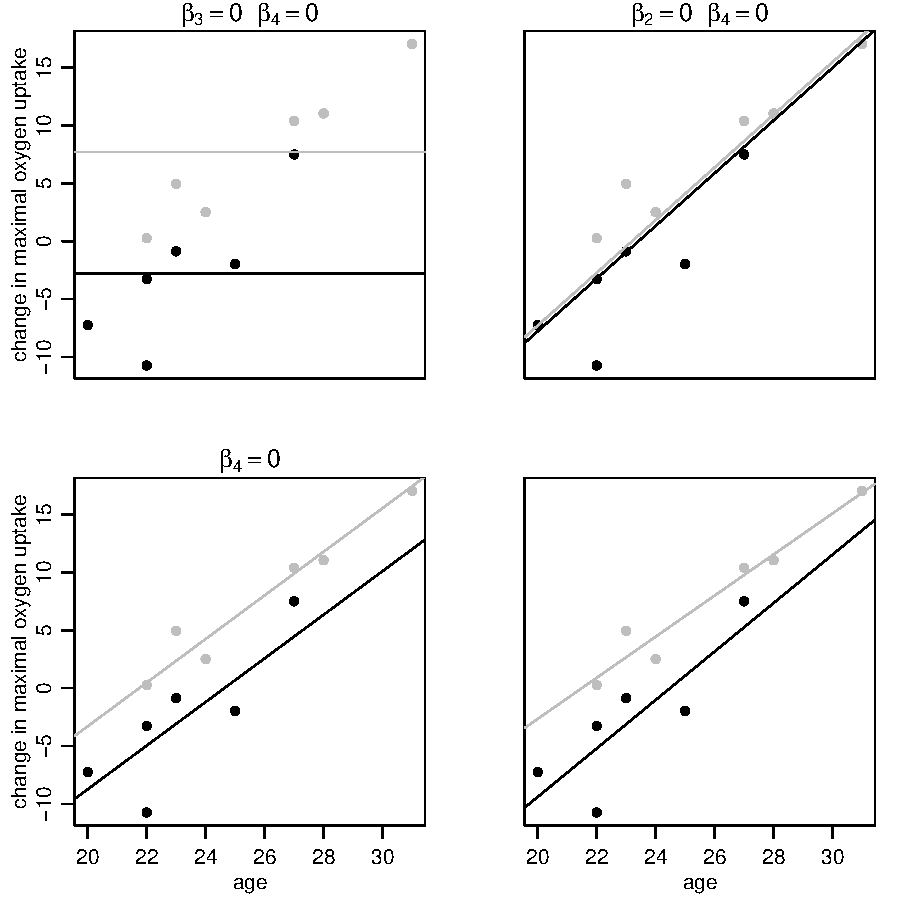
\includegraphics{Regression-003}

Let's find the least squares regression estimates for the model in \ref{example_model}, and use the results to evaluate the differences between the two exercise groups.  The ages of the 12 subjects, along with their observed changes in maximal oxygen uptake, are

\begin{flalign*}
    \mathbf{x}_3 &= (23,22,22,25,27,20,31,23,27,28,22,24)\\
    \mathbf{y}   &= (-0.87,-10.74,-3.27,-1.97,7.50,-7.25,17.05,4.96,10.40,11.05,0.26,2.51),
\end{flalign*}

\noindent with the first six elements of each vector corresponding to the subjects in the running group and the latter six corresponding ot sujects in the aerobics group.  After constructing the $12 \time 4$ matrix $\mathbf{X}$ out of the vectors $\mathbf{x}_1,\mathbf{x}_2,\mathbf{x}_3,\mathbf{x}_4$ defined as in (\ref{example_model}), the matrices $\mathbf{X}^T\mathbf{X}$ and $\mathbf{X}^T\mathbf{y}$ can be computed, from which we get $\beta_{ols} = (-51.29,13.11,2.09,-0.32)^T$:\\



\begin{Schunk}
\begin{Sinput}
> n <- length(y)
> x1 <- rep(1,n)
> x4 <- x2*x3
> X = cbind(x1,x2,x3,x4)
> p = ncol(X)
> beta.ols<- solve(t(X)%*%X)%*%t(X)%*%y
> sig2.ols = (t(y-X%*%beta.ols)%*%(y-X%*%beta.ols)/(n-p))[1]
> sig2.ols
\end{Sinput}
\begin{Soutput}
[1] 8.542477
\end{Soutput}
\begin{Sinput}
> #sampling variance-covariance matrix of beta.ols:
> SIG2.ols = solve(t(X)%*%X)*sig2.ols
> #standard errors for the components of beta.ols:
> SE.ols = sqrt(diag(SIG2.ols))
> betadata = cbind(beta.ols,SE.ols)
> colnames(betadata) = c("beta.ols","SE.ols")
> betadata
\end{Sinput}
\begin{Soutput}
      beta.ols     SE.ols
x1 -51.2939459 12.2522126
x2  13.1070904 15.7619762
x3   2.0947027  0.5263585
x4  -0.3182438  0.6498086
\end{Soutput}
\end{Schunk}

This means that the estimated linear relationship between uptake and age has an intercept and slope of -51.29 and 2.09 for the running group, and -51.29 + 13.11 = -38.18 and 2.09 - 0.32 = 1.77 for the aerobics group.  These two lines are plotted in the fourth panel of Figure XX.  We obtain unbiased estimate $\sigma^2 = SSR(\hat{\beta}_{ols})/(n-p) = 8.54$, and use this to compute the standard error of the components of $\hat{\beta}_{ols}$, which are 12.25, 15.76, 0.53, and 0.65, respectively.  comparing the values of $\hat{\beta}_{ols}$ to their standard errors suggests that the evidence for differences between the two exercise regimens is not very strong.

\clearpage



\end{document}
